\section{Allgemeine Übersicht}

\textit{
Domino's Pizza® dominiert die Dystopie Düsburgs.
Kann Pizza Hut® den Ruf der runden Fressalien retten?
Begib dich zur Auslieferung an die Front und beweise deine italienischen Wurzeln!
}

Das Spiel \textit{Pizza Hut 2077} ist ein Sidescolling Jump'n'Run.
Das Spiel besteht aus einer simplen 2-Dimensionalen Welt.
Diese ist mit zufällig generierten Plattformen gefüllt.
Das konkrete Ziel des Spiels besteht lediglich in dem Highscore.
Während des Ablaufes muss der Spieler Gegnern ausweichen und sich von Platform zu Platform hangeln.
Der Spieler kann diese Gegner durch das Werfen von Pizzen eliminieren.
Die Feuerrate der Pizzen ist jedoch limitiert.
Das Spiel ist zu Ende, wenn der Spieler von einem Gegner berührt wird oder aus der Welt fällt (bzw. nicht auf einer Platform landet).
Alle dem Genre üblichen Funktionen sind wie zu erwarten realisiert.

Am Ende des Spiels kann der Spieler seinen Highscore mitsamt einem Namen in einer Datenbank speichern.
Die \gls{mysql} Datenbank ist online gehosted, darum wird eine funktionierende Internetverbindung benötigt.
In dem Credits-Bildschirm kann, mit dem notwendigen Administrator Passwort, die Highscore Tabelle der Datenbank zurückgesetzt werden.
Das einfügen von neuen Highscores zum Spielende verläuft ohne Passwort.
Die Dateneingabe hat jedoch nur Rechte zum Erstellen neuer Daten und ist auch gegen \texttt{SQL}-Injections gehärtet.

Die Hintergrundmusik des Spiels reagiert auf den jeweiligen Zustand.
Im Hauptmenü wird eine ruhigere Version des Arpeggio Leitmotivs gespielt.
Zum Spielstart geht diese mit über eine Brücke in den Hauptteil über.
Der Hauptteil wird während des Spielverlaufs gelooped.
Wenn der Spieler stirbt, wird der Hauptteil durch das Outtro unterbrochen.
Der Soundtrack stammt aus eigener Komposition.
Außerdem haben die Aktionen des Spielers zugehörige Soundeffekte, wie beispielsweise beim Springen oder bei dem Werfen von Pizzen, die passend abgespielt werden.

Die Graphik des Spiels beruhen auf \gls{jfx}.
Die meisten graphischen Elemente und Animationen sind durch individuelle Sprites implementiert.
Einfache Animationen wurde durch das Abspielen verschiedener Sprites nacheinander realisiert.
Alle Sprites stammen aus eigener Produktion.
Interaktive Elemente wie Text und Eingabefelder nutzen jedoch \gls{jfx} Widgets.

Das Projekt wird mithilfe von \gls{maven} kompiliert.
Zur Ausführung ist eine funktionierende Instanz davon nicht notwendig, lediglich eine \gls{jre} von Version 18 oder später.
Da das Projekt in eine eigenständige \gls{jar} mitsamt aller Ressourcen (Sprites und Sounds) und aller notwendigen Abhängigkeiten (\gls{jfx} und Freunde) kompiliert werden kann.
Außerdem kann durch \gls{maven} eine vollwertige und interaktive Dokumentation mit \gls{javadoc} erstellt werden.
Die gesamte Codebase ist auch in der \gls{javadoc} Konvention kommentiert.

Anleitungen zur Kompilation, Steuerung und Tasten und weiteres können in der \texttt{README.md} gefunden werden.
Attribution für benutzte Ressourcen ist in der \texttt{ATTRIBUTION.md} gelistet.

\subsection{\acrshort{uml}-Diagramm}

\begin{figure}[H]
    \centering
    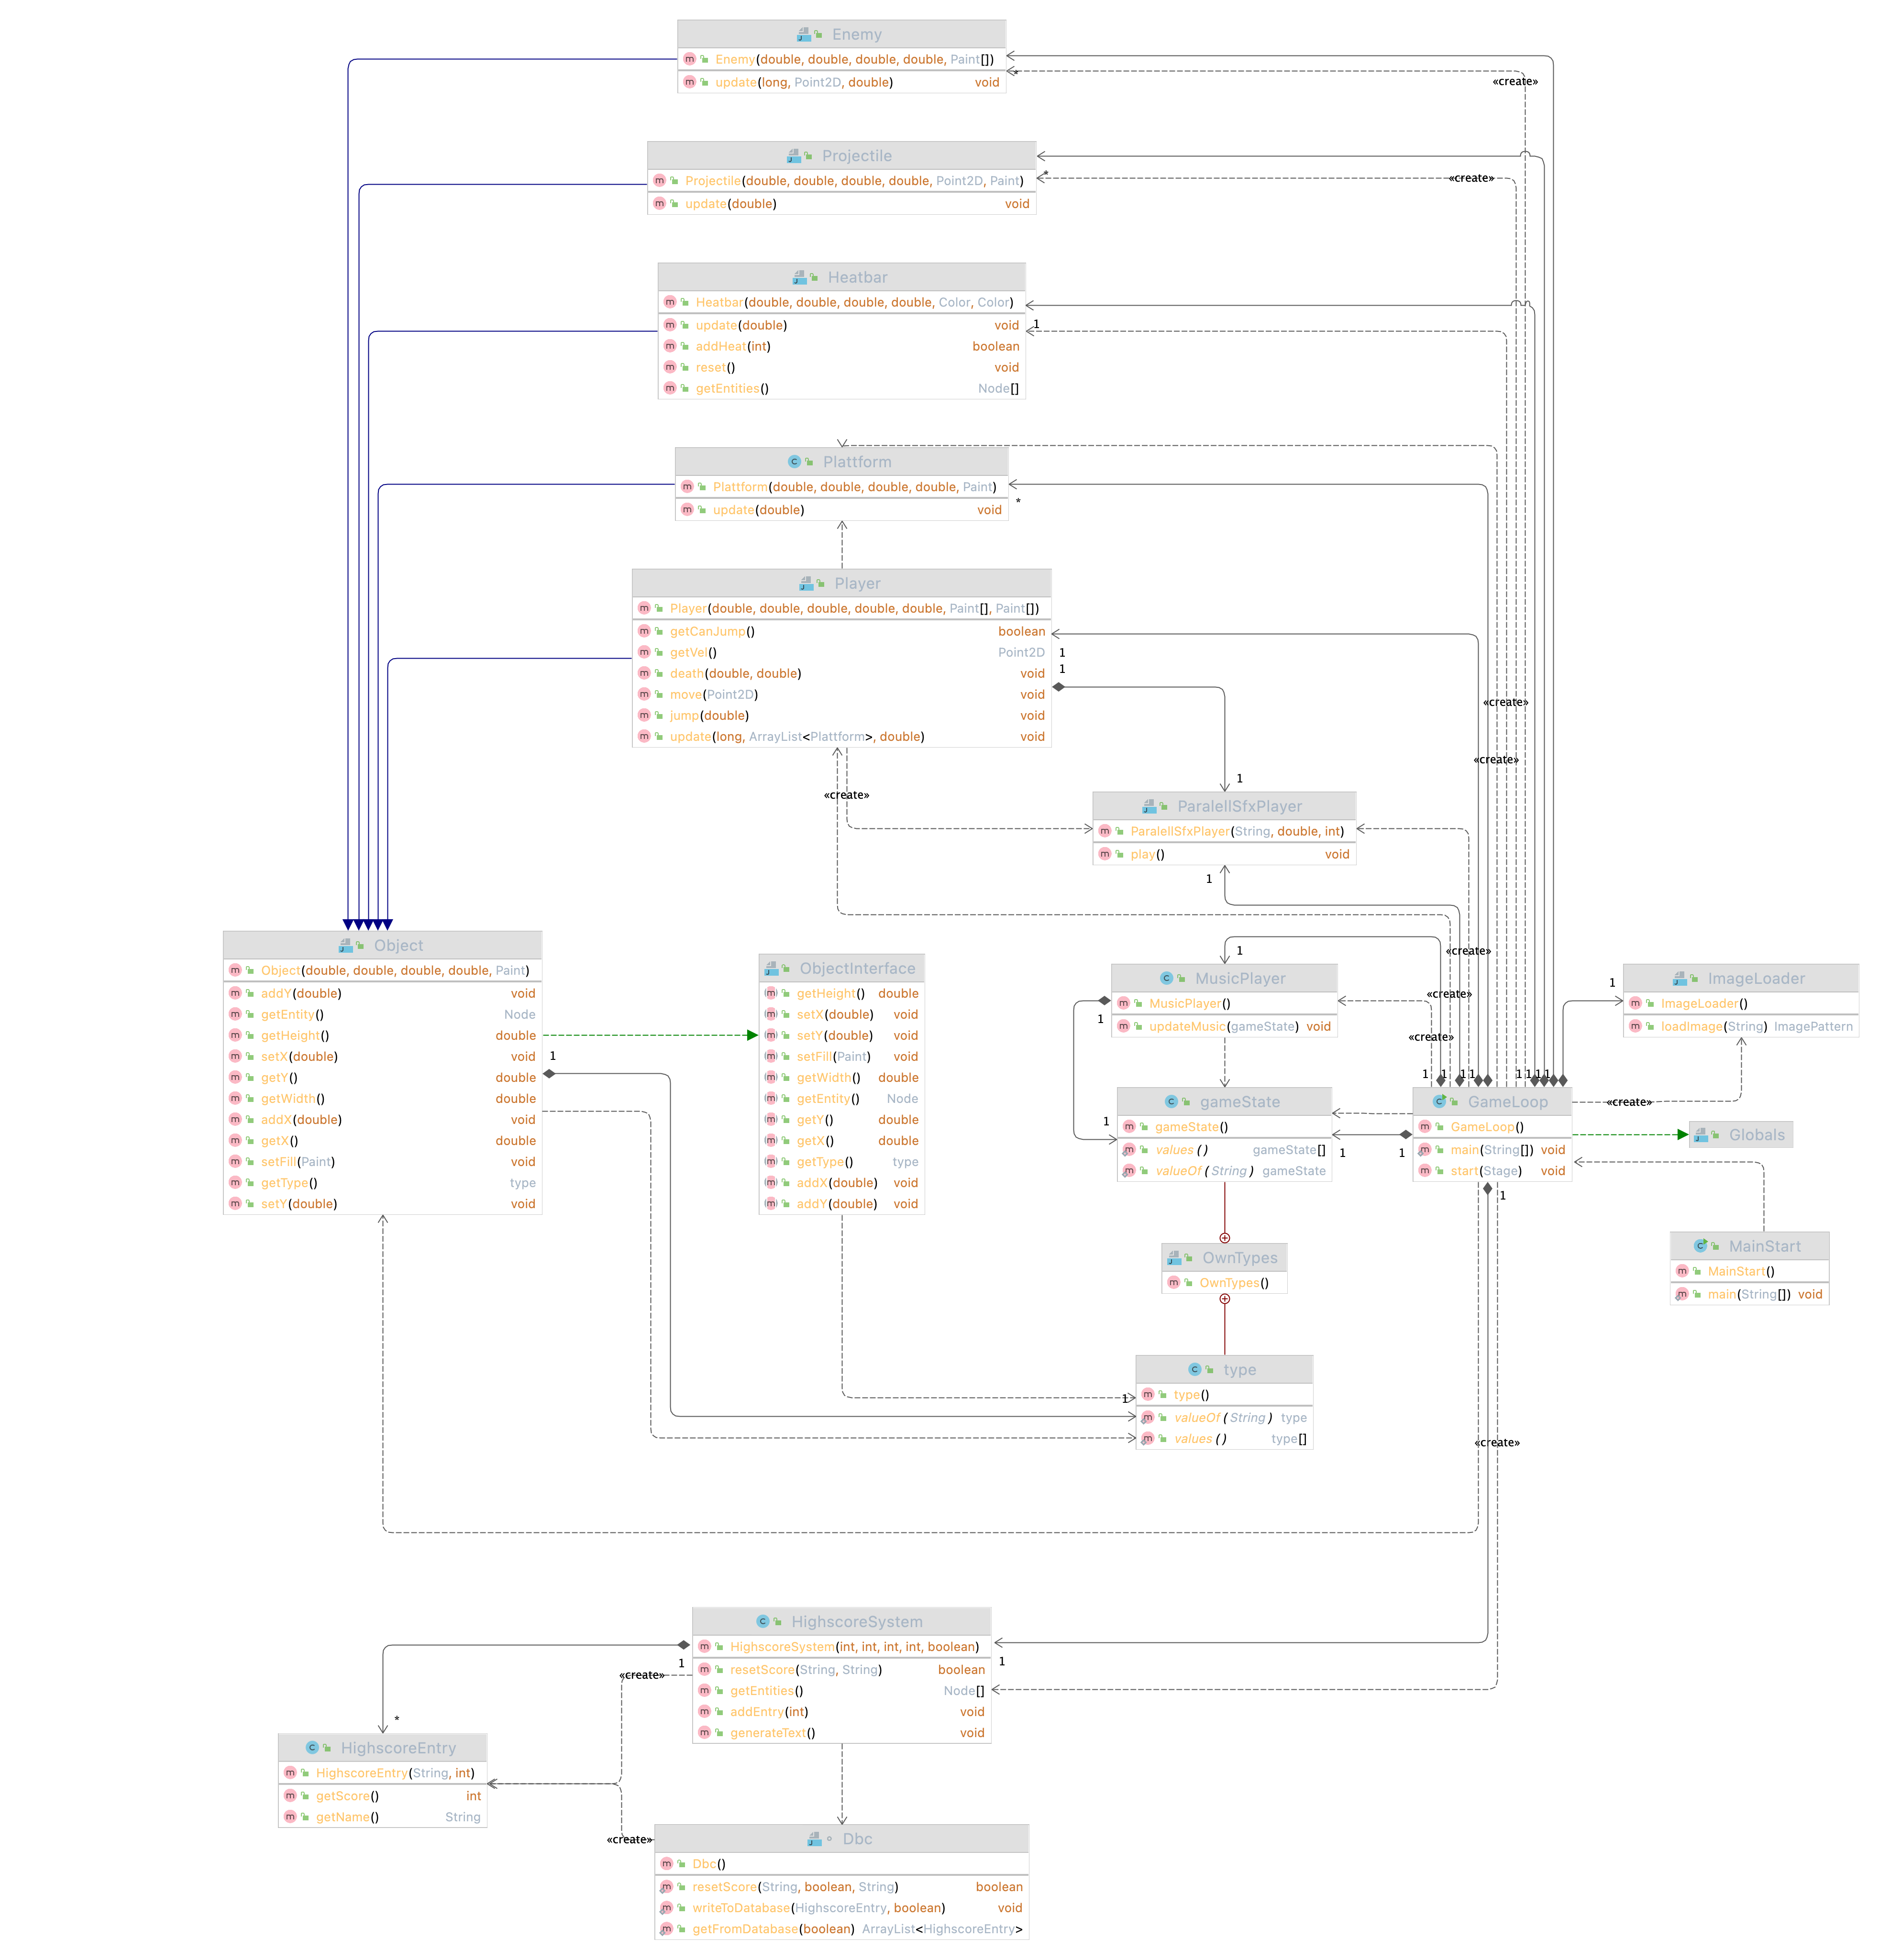
\includegraphics[width=0.9\textwidth]{../../uml-light.png}
    \caption{\gls{uml}-Diagramm des Projekts. Das Bild befindet sich auch im Haupt-Verzeichniss des Projekts.}
    \label{fig:uml}
\end{figure}

Das ist \autoref{fig:uml} dargestellte \gls{uml} Diagramm gibt den gesamten Inhalt des implementierten Projekts an.
Äußere Abhängigkeiten werden nicht aufgeführt.
Der Großteil spielt sich in und um der Klasse \texttt{GameLoop} ab.
Die relevanten Teile der Core-Gameplay-Schleife und weiteres werden darin erstellt und aktualisiert.
Alle im Spiel auftretenden Elemente erben von der Klasse \texttt{Objekt}, welche das \texttt{ObjectInterface} implementiert.
Musik wird durch die \texttt{MusicPlayer} Klasse gehandhabt und Sound durch den \texttt{ParralellSFXPlayer}.
Bilder und Graphiken werden durch den \texttt{ImageLoader} geladen aber von den Verbrauchern selbst verwaltet.
Das Highscore System mitsamt der Datenbank Verbindung wird in \texttt{HighscoreSystem}, \texttt{HighscoreEntry} und \texttt{DBC} (DataBase Connection) implementiert.
Die Klasse \texttt{MainStart} ist eine Helferklasse um die \gls{jfx} Applikation zu initialisieren.
